%___________________________________________________________________________

\hypertarget{monte-carlo-methods-in-bayesian-analysis}{}
\pdfbookmark[0]{Monte Carlo Methods in Bayesian Analysis}{monte-carlo-methods-in-bayesian-analysis}

\section*{Monte Carlo Methods in Bayesian Analysis}

Bayesian model specification often results in posterior forms that are difficult to manipulate analytically. However, it is often possible to generate simulated values that share the distributional properties of the specified posterior. Such simulations may be summarized in such a way that describes the posterior density. For example, consider the expected value of some integral quantity:

\[
E[{\bf x}] = \int_{-\infty}^{\infty} {\bf x} f({\bf x}) d{\bf x}, \qquad
{\bf x} = \{x_1,...,x_k\}
\]

\noindent where $k$ is perhaps very large, making the joint distribution of ${\bf x}$ analytically complex. If we can produce random vectors $\{{\bf x_i}\}$, we can use these values to approximate the unknown integral. This process is known as {\emph Monte Carlo integration}. In general, MC integration says that:

\[
I[a,b] = \int_a^b h(x) f(x) dx
\]

\noindent can be estimated by:

\[
\hat{I}[a,b] = \frac{1}{n}\sum_{i=1}^n h(x_i)
\]

\noindent This estimate is useful because:

\begin{itemize}
\item
By the strong law of large numbers:
\[\hat{I}[a,b] \rightarrow I[a,b] \mbox{with probability 1}\]
\item
Simulation error can be measured and controlled:
\[Var(\hat{I}[a,b]) = \frac{1}{n(n-1)}\sum_{i=1}^n (h(x_i)-\hat{I}[a,b])^2\]
\end{itemize}

Why is this relevant to Bayesian analysis? If we replace $f(x)$ with a posterior, $\pi(\theta|x)$ and make $h(x)$ an interesting function of the unknown stoch, the resulting expectation is that of the posterior of $h(\theta)$:

\[
E[h(\theta|x)] = \int \pi(\theta|x) h(\theta) d\theta \approx \frac{1}{n}\sum_{i=1}^n h(\theta)
\]

%___________________________________________________________________________

\hypertarget{rejection-sampling}{}
\pdfbookmark[1]{Rejection Sampling}{rejection-sampling}
\subsection*{Rejection Sampling}

Though Monte Carlo integration allows us to estimate integrals that are unassailable by analysis, it relies on the ability to draw samples from the posterior distribution. For known stochetric forms, this is not a problem; probability integral transforms or bivariate techniques (e.g Box-Muller method) may be used to obtain samples from uniform pseudo-random variates generated from a computer. Often, however, we cannot readily generate random values from non-standard posteriors. In such instances, we can use rejection sampling to generate samples.

\begin{figure}[ht]
        \begin{center}
        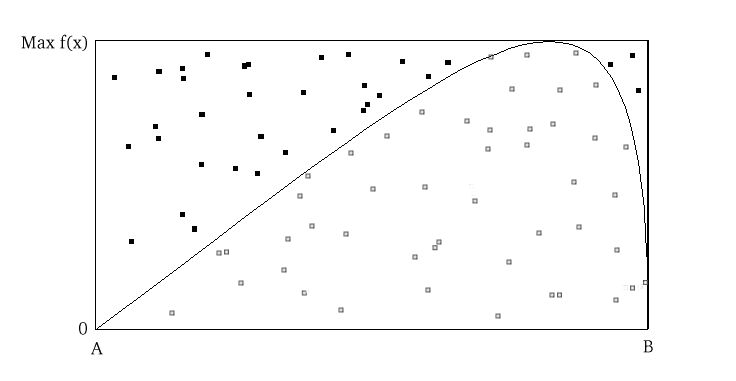
\includegraphics[scale=0.4]{reject.png}
    \end{center}
    \caption{Rejection sampling of a bounded form. Area is estimated by the ratio of accepted (open squares) to total points, multiplied by the rectangle area.}
    \label{fig:bound}
\end{figure}

Posit a function, $f(x)$ which can be evaluated for any value on the support of $x:S_x = [A,B]$, but may not be integrable or easily sampled from. If we can calculate the maximum  value of $f(x)$, we can then define a rectangle that is guaranteed to contain all possible values $(x,f(x))$. It is then trivial to generate points over the box and enumerate the values that fall under the curve (Figure \ref{fig:bound}).

\[
\frac{\mbox{Points under curve}}{\mbox{Points generated}} \times \mbox{box area} = \lim_{n \to \infty} \int_A^B f(x) dx
\]

\begin{figure}[h]
        \begin{center}
        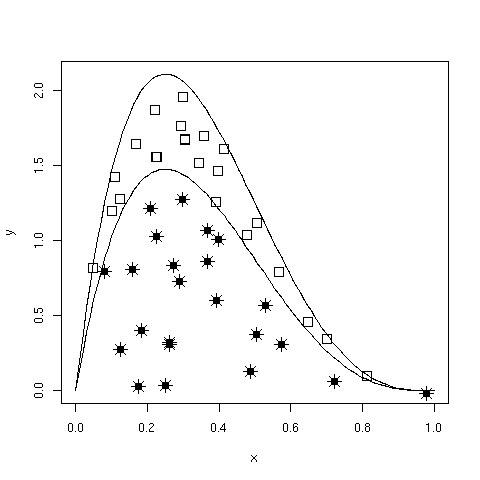
\includegraphics[scale=0.4]{envelope.png}
    \end{center}
    \caption{Rejection sampling of an unbounded form using an enveloping distribution.}
    \label{fig:unbound}
\end{figure}

\noindent This approach is useful, for example, in estimating the normalizing constant for posterior distributions.

If $f(x)$ has unbounded support (i.e. infinite tails), such as a Gaussian distribution, a bounding box is no longer appropriate. We must specify a majorizing (or, enveloping) function, $g(x)$, which implies:

\[
g(x) \le  f(x) \qquad\forall x \in (-\infty,\infty)
\]

Having done this, we can now sample ${x_i}$ from $g(x)$ and accept or reject each of these values based upon $f(x_i)$. Specifically, for each draw $x_i$, we also draw a uniform random variate $u_i$ and accept $x_i$ if $u_i < f(x_i)/kg(x_i)$ (Figure \ref{fig:unbound}). This approach is made more efficient by choosing an enveloping distribution that is ``close'' to the target distribution, thus maximizing the number of accepted points. Further improvement is gained by using optimized algorithms such as importance sampling (see text) which, as the name implies, samples more frequently from important areas of the distribution.

%___________________________________________________________________________

\hypertarget{markov-chains}{}
\pdfbookmark[0]{Markov Chains}{markov-chains}
\section*{Markov Chains}

A Markov chain is a special type of \emph{stochastic process}. The standard definition of a stochastic process is an ordered collection of random variables:

\[
\{X_t:t \in T\}
\]

\noindent where $t$ is frequently (but not necessarily) a time index. If we think of $X_t$ as a state $X$ at time $t$, and invoke the following dependence condition on each state:

\[
Pr(X_{t+1}=x_{t+1} | X_t=x_t, X_{t-1}=x_{t-1},\ldots,X_0=x_0) = Pr(X_{t+1}=x_{t+1} | X_t=x_t)
\]

\noindent then the stochastic process is known as a Markov chain. This conditioning specifies that the future depends on the current state, but not past states. Thus, the Markov chain wanders about the state space, remembering only where it has just been in the last time step. The collection of transition probabilities is sometimes called a \emph{transition matrix} when dealing with discrete states, or more generally, a \emph{transition kernel}. In the context of Markov chain Monte Carlo, useful to think of the Markovian property as ``mild non-independence''\footnote{In general, for Bayesian analyses, statistical independence is less relevant, relative to classical statistical inference. Instead, we substitute the notion of \emph{exchangeability}, which is a weaker concept, but often just as useful. Exchangeability essentially implies that different permutations (orderings) of a sequence of random variables will have the same marginal distribution. A sequence of random quantities may not be considered independent in a Bayesian sense, but are frequently exchangeable.}. We will see that, while it may be difficult to generate independent samples from a particular posterior distribution, it may be possible to generate dependent samples that may be useful in describing that distribution.

%___________________________________________________________________________

\hypertarget{jargon-busting}{}
\pdfbookmark[1]{Jargon-busting}{jargon-busting}
\subsection*{Jargon-busting}

Before we move on, it is important to define some general properties of Markov chains. They are frequently encountered in the MCMC literature, and some will help us decide whether MCMC is producing a useful sample from the posterior.

\begin{itemize}
\item \emph{Homogeneity}: A Markov chain is homogeneous at step $t$ if the transition probabilities are independent of the state at $t$. The starting point of the chain is almost never homogeneous, as the initial values are either hand-picked or arbitrary.
\item \emph{Irreducibility}: A Markov chain is irreducible if every state is accessible in one or more steps from any other state. That is, the chain contains no absorbing states. This implies that there is a non-zero probability of eventually reaching state $k$ from any other state in the chain.
\item \emph{Recurrence}: States which are visited repeatedly are \emph{recurrent}. If the expected time to return to a particular state is bounded, this is known as \emph{positive recurrence}, otherwise the recurrent state is \emph{null recurrent}. Further, a chain is \emph{Harris recurrent} when it visits all states $X \in S$ infinitely often in the limit as $t \to \infty$; this is an important characteristic when dealing with unbounded, continuous state spaces. Whenever a chain ends up in a closed, irreducible set of Harris recurrent states, it stays there forever and visits every state with probability one.
\item \emph{Stationarity}: A stationary Markov chain produces the same marginal distribution when multiplied by the transition kernel.  Thus, if $P$ is some $n \times n$ transition matrix:

\[{\bf \pi P} = {\bf \pi}\]

\noindent for Markov chain $\pi$. Thus, $\pi$ is no longer subscripted, and is referred to as the \emph{limiting distribution} of the chain. In MCMC, the chain explores the state space according to its limiting marginal distribution.
\item \emph{Ergodicity}: Ergodicity is an emergent property of Markov chains which are irreducible, positive Harris recurrent and aperiodic. Ergodicity is defined as:

\[
\lim_{n \to \infty} Pr^{(n)}(\theta_i,\theta_j) = \pi(\theta_j) \quad \forall \theta_i, \theta_j \in \Theta
\]

\noindent or in words, the marginal distribution of the chain is the same at one step as at all other steps. This implies that our Markov chain, which we recall is dependent, now generates quantities that are independent. If it means anything to you, ergodicity is the analogue of the strong law of large numbers for Markov chains. For example, take values $\theta_{i+1},\ldots,\theta_{i+n}$ from a chain that has reached an ergodic state. A statistic of interest can then be estimated by:

\[
\hat{h}(\theta) = \frac{1}{n}\sum_{j=i+1}^{i+n} h(\theta_j) \approx h(\theta)
\]

\end{itemize}

%___________________________________________________________________________

\hypertarget{reversible-markov-chains}{}
\pdfbookmark[0]{Why MCMC Works: Reversible Markov Chains}{reversible-markov-chains}
\section*{Why MCMC Works: Reversible Markov Chains}

Markov chain Monte Carlo simulates a Markov chain for which some function of interest (\emph{e.g.} the joint distribution of the stochs of some model) is the unique, invariant limiting distribution. An invariant distribution with respect to some Markov chain with transition kernel $Pr(y \mid x)$ implies that:
\[
\int_x Pr(y \mid x) \pi(x) dx = \pi(y),
\]
and similarly:
\[
\int_y Pr(x \mid y) \pi(y) dy = \pi(x),
\]

Invariance is guaranteed for any \textbf{reversible} Markov chain. Consider a Markov chain in reverse sequence: $\{\theta^{(n)},\theta^{(n-1)},...,\theta^{(0)}\}$. This sequence is still Markovian, because:
\[
Pr(\theta^{(k)}=y \mid \theta^{(k+1)}=x,\theta^{(k+2)}=x_1,\ldots ) = Pr(\theta^{(k)}=y \mid \theta^{(k+1)}=x)
\]
Forward and reverse transition probabilities may be related through Bayes theorem:
\begin{eqnarray}
Pr(\theta^{(k)}=y \mid \theta^{(k+1)}=x) &=& \frac{Pr(\theta^{(k+1)}=x \mid \theta^{(k)}=y) Pr(\theta^{(k)}=y)}{Pr(\theta^{(k+1)}=x)} \nonumber \\
&=& \frac{Pr(\theta^{(k+1)}=x \mid \theta^{(k)}=y) \pi^{(k)}(y)}{\pi^{(k+1)}(x)} \nonumber
\end{eqnarray}

\[
\frac{Pr(\theta^{(k+1)}=x \mid \theta^{(k)}=y) \pi^{(k)}(y)}{\pi^{(k+1)}(x)}
\]

\noindent Though not homogeneous in general, $\pi$ becomes homogeneous if:
\begin{itemize}
\item $n \rightarrow \infty$
\item $\pi^{(0)}=\pi$ for some $i < k$
\end{itemize}

\noindent If this chain is homogeneous it is called reversible, because it satisfies the \textbf{detailed balance equation}:
\[
\pi(x)Pr(y \mid x) = \pi(y) Pr(x \mid y)
\]
Reversibility is important because it has the effect of balancing movement through the entire state space. When a Markov chain is reversible, $\pi$ is the unique, invariant, stationary distribution of that chain.
Hence, if $\pi$ is of interest, we need only find the reversible Markov chain for which $\pi$ is the limiting distribution. This is what MCMC does!

%___________________________________________________________________________

\hypertarget{gibbs-sampling}{}
\pdfbookmark[0]{Gibbs Sampling}{gibbs-sampling}
\section*{Gibbs Sampling}

The Gibbs sampler is the simplest and most prevalent MCMC algorithm. It uses samples from conditionally independent distributions to generate a sample from the fully conditional Bayesian posterior. For example, if a posterior has $k$ stochs to be estimated, we may condition each stoch on current values of the other $k-1$ stochs, and sample from the resultant distributional form (usually easier), and repeat this operation on the other stochs in turn. Note that we have now combined Markov chains (conditional independence) and Monte Carlo techniques (estimation by simulation) to yield Markov chain Monte Carlo.

Here is a stereotypical Gibbs sampling algorithm:

\newcounter{lcount}
\begin{list}{\arabic{lcount}}
{\usecounter{lcount}}
\item Choose starting values for states (stochs): ${\bf \theta} = [\theta_1^{(0)},\theta_2^{(0)},\ldots,\theta_k^{(0)}]$
\item Initialize counter $j=1$
\item Draw the following values from each of the $k$ conditional distributions:
\begin{eqnarray*}
\theta_1^{(j)} &\sim& \pi(\theta_1 | \theta_2^{(j-1)},\theta_3^{(j-1)},\ldots,\theta_{k-1}^{(j-1)},\theta_k^{(j-1)}) \\
\theta_2^{(j)} &\sim& \pi(\theta_2 | \theta_1^{(j)},\theta_3^{(j-1)},\ldots,\theta_{k-1}^{(j-1)},\theta_k^{(j-1)}) \\
\theta_3^{(j)} &\sim& \pi(\theta_3 | \theta_1^{(j)},\theta_2^{(j)},\ldots,\theta_{k-1}^{(j-1)},\theta_k^{(j-1)}) \\
\vdots \\
\theta_{k-1}^{(j)} &\sim& \pi(\theta_{k-1} | \theta_1^{(j)},\theta_2^{(j)},\ldots,\theta_{k-2}^{(j)},\theta_k^{(j-1)}) \\
\theta_k^{(j)} &\sim& \pi(\theta_k | \theta_1^{(j)},\theta_2^{(j)},\theta_4^{(j)},\ldots,\theta_{k-2}^{(j)},\theta_{k-1}^{(j)})
\end{eqnarray*}
\item Increment $j$ and repeat until convergence occurs.
\end{list}

As we can see from the algorithm, each distribution is conditioned on the last iteration of its chain values, constituting a Markov chain as advertised. The Gibbs sampler has all of the important properties outlined in the previous section: it is aperiodic, homogeneous and ergodic. Once the sampler converges, all subsequent samples are from the target distribution. This convergence occurs at a geometric rate.

Implementing a simple Gibbs sampler can be done easily in Python. Lets build a Gibbs sampler for estimating a single stoch; for example, simulating from a binomial distribution with a beta prior for $p$ (we assume $n$ is known). We just need a random number generator and a simple loop to iterate over each stoch:
\vspace{1cm}
\begin{verbatim}
# Import random number generators
from numpy import random
beta = random.beta
binomial = random.binomial

# Number of iterations
k=1000

# Prior stoch values
n=20
a=1
b=2

# Some fake data
data = [6,8,4,9,9,7,12]

# Empty arrays to store output
plist = []
ylist = []

# Here's the sampler
for i in range(k):

     # Sample from beta distribution
    p = beta(a+sum(data), len(data)*n-sum(data)+b)

    # Sample from binomial distribution
    y = binomial(n,p)

     # Append samples to lists
    plist.append(p)
    ylist.append(y)

# Calculate medians
plist.sort()
ylist.sort()
pmed = (plist[k/2]+plist[k/2+1])/2
ymed = (ylist[k/2]+ylist[k/2+1])/2

# Print results
print pmed, ymed
\end{verbatim}
\vspace{1cm}

%___________________________________________________________________________

\hypertarget{the-metropolis-hastings-algorithm}{}
\pdfbookmark[0]{The Metropolis-Hastings Algorithm}{the-metropolis-hastings-algorithm}
\section*{The Metropolis-Hastings Algorithm}

The key to success in applying the Gibbs sampler to the estimation of Bayesian posteriors is being able to specify the form of the complete conditionals of ${\bf \theta}$. In fact, the algorithm cannot be implemented without them. Of course, the posterior conditionals cannot always be neatly specified. The Metropolis-Hastings algorithm, which is implemented by PyMC, rather than generating values from the full set of conditionals, generates candidate state transitions from an alternate distribution, and accepts or rejects each candidate probabilistically according to a specified acceptance ratio.

Let us first consider a simple Metropolis-Hastings algorithm for a single stoch, $\theta$. If necessary, we can transform $\theta$ so that its distribution $\pi(\theta)$ has support over the real line, $\theta:S_{\theta} = (-\infty,\infty)\}$, facilitating the use of convenient random variables such as the normal. This sampling distribution will be used to produce candidate variables, and is therefore referred to as the \emph{proposal distribution}, $q_t(\theta^{\prime} | \theta)$. That is, the generated value, $\theta^{\prime}$, is a \emph{possible} next value for $\theta$ at step $t+1$. We also need to be able to calculate the probability of moving back to the original value from the candidate, or $q_t(\theta | \theta^{\prime})$. These probabilistic ingredients are used to define an \emph{acceptance ratio}:

\[
a(\theta^{\prime},\theta) = \frac{q_t(\theta^{\prime} | \theta) \pi(\theta^{\prime})}{q_t(\theta | \theta^{\prime}) \pi(\theta)}
\]

\noindent The value of $\theta^{(t+1)}$ is then determined by:

\[
\theta^{(t+1)} = \left\{\begin{array}{l@{\quad \mbox{with prob.} \quad}l}\theta^{\prime} & \min(a(\theta^{\prime},\theta),1) \\ \theta^{(t)} & 1 - \min(a(\theta^{\prime},\theta),1) \end{array}\right.
\]

\noindent This transition kernel implies that movement is not guaranteed at every step. It only occurs if the suggested transition is likely based on the acceptance ratio.

A single iteration of the Metropolis-Hastings algorithm proceeds as follows:

\newcounter{lcount2}
\begin{list}{\arabic{lcount2}}
{\usecounter{lcount2}}
\item Sample $\theta^{\prime}$ from $q(\theta^{\prime} | \theta^{(t)})$.
\item Generate a Uniform[0,1] random variate $u$.
\item If $a(\theta^{\prime},\theta) > u$ then $\theta^{(t+1)} = \theta^{\prime}$, otherwise $\theta^{(t+1)} = \theta^{(t)}$.
\end{list}

\noindent The original form of the algorithm specified by Metropolis required that $q_t(\theta^{\prime} | \theta) = q_t(\theta | \theta^{\prime})$, which reduces $a(\theta^{\prime},\theta)$ to $\pi(\theta^{\prime})/\pi(\theta)$, but this is not necessary. In either case, the state moves to high-density points in the distribution with high probability, and to low-density points with low probability. After convergence, the Metropolis-Hastings algorithm describes the full target posterior density, so all points are recurrent.

%___________________________________________________________________________

\hypertarget{random-walk-metropolis-hastings}{}
\pdfbookmark[1]{Random-walk Metropolis-Hastings}{random-walk-metropolis-hastings}
\subsection*{Random-walk Metropolis-Hastings}

A practical implementation of the Metropolis-Hastings algorithm makes use of a random-walk proposal. Recall that a random walk is a Markov chain that evolves according to:

\begin{eqnarray*}
\theta^{(t+1)} &=& \theta^{(t)} + \epsilon_t \\
\epsilon_t &\sim& f(\phi)
\end{eqnarray*}

As applied to the MCMC sampling, the random walk is used as a proposal distribution, whereby dependent proposals are generated according to:

\[
q(\theta^{\prime} | \theta^{(t)}) = f(\theta^{\prime} - \theta^{(t)}) = \theta^{(t)} + \epsilon_t
\]

Generally, the density generating $\epsilon_t$ is symmetric about zero, resulting in a symmetric chain. Chain symmetry implies that $q(\theta^{\prime} | \theta^{(t)}) = q(\theta^{(t)} | \theta^{\prime})$, which reduces the Metropolis-Hastings acceptance ratio to:

\[
a(\theta^{\prime},\theta) = \frac{\pi(\theta^{\prime})}{\pi(\theta)}
\]

The choice of the random walk distribution for $\epsilon_t$ is frequently a normal or Student's $t$ density, but it may be any distribution that generates an irreducible proposal chain.

An important consideration is the specification of the scale stoch for the random walk error distribution. Large values produce random walk steps that are highly exploratory, but tend to produce proposal values in the tails of the target distribution, potentially resulting in very small acceptance rates. Conversely, small values tend to be accepted more frequently, since they tend to produce proposals close to the current stoch value, but may result in chains that mix very slowly. Some simulation studies suggest optimal acceptance rates in the range of 20-50\%. It is often worthwhile to optimize the proposal variance by iteratively adjusting its value, according to observed acceptance rates early in the MCMC simulation.
